\documentclass[a4paper,12pt]{article} 
\usepackage[T2A]{fontenc}			
\usepackage[utf8]{inputenc}			
\usepackage[english,russian]{babel}
\usepackage{float}
\usepackage{amsmath,amsfonts,amssymb,amsthm,mathrsfs,mathtools} 
\usepackage{cancel}
\usepackage{multirow}
\usepackage[colorlinks, linkcolor = blue]{hyperref}
\usepackage{upgreek}\usepackage[left=2cm,right=2cm,top=2cm,bottom=3cm,bindingoffset=0cm]{geometry}
\usepackage{tikz}
\usepackage{graphicx}
\usepackage{subfig}
\usepackage{titletoc}
\usepackage{pgfplots}
\usepackage{xcolor}
\usepackage{wrapfig}
\usepackage{pgfplots}
\pgfplotsset{width=10cm,compat=1.9}

\begin{document}

\begin{titlepage}
		\vspace*{\fill}
		
		\begin{center}
			
\includegraphics[scale=0.8]{MIPT.pdf}
			\\[0.7cm]\Huge Московский Физико-Технический Институт
			\\[2cm]\LARGE Отчет по эксперименту
			\\[0.5cm]\noindent\rule{\textwidth}{1pt}
			\\\Huge\textbf{4.5.2. \\ Интерференция лазерного излучения}
			\\[-0.5cm]\noindent\rule{\textwidth}{1pt}
		\end{center}
		
		\vspace*{\fill}
		
		\begin{flushleft}
			Выполнила: \hspace{\fill} Группа:
			\\Малиновская София \hspace{\fill} Б05-102
		\end{flushleft}
	\end{titlepage}

	\setcounter{page}{2}

\section*{Цель работы} 
Исследовать зависимость видности интерфереционной картины от разности хода интерферирующих лучей и от их поляризации.

\section*{В работе используются}
He-Ne лазер, интерферометр Майкельсона с подвижным зеркалом, фотодиод с усилителем, осциллограф С1-76, поляроид, линейка.
\section*{Теоретическая сводка}
\paragraph*{Гелий-неоновый лазер}
Лазер представляет собой интерферометр Фабри-Перо -- газовую трубку с двумя параллельными зеркалами по обе стороны. Пусть $\Delta F$ -- половина диапазона генерации лазера, а $\Delta \nu$ -- межмодовое расстояние. Тогда межмодовое расстояние выражается как
\begin{equation}
    \Delta \nu = \dfrac{c}{2L}
\end{equation}
При этом число мод можно оценить как 
\begin{equation}
N \approx 1 + \dfrac{2\Delta F}{\Delta \nu}.
\end{equation}
\paragraph*{Видимость}
Видимость интерфереционной картины -- параметр, определяемый формулой
\begin{equation}
\gamma = \dfrac{I_{max} - I_{min}}{I_{max} + I_{min}},
\end{equation}
где $I_{max}$, $I_{min}$ -- максимальная и минимальная интенсивности света интерфереционной картины вблизи выбранной точки. Разобьём его на произведение функций параметров установки
$$
\gamma = \gamma_1 \gamma_2 \gamma_3.
$$
Здесь $\gamma_1$
\begin{equation}
\gamma_1 = \dfrac{2\sqrt{\delta}}{1+\delta},
\end{equation}
где $\delta = \frac{B_m^2}{A_m^2}$, $A_m^2$ и $B_m^2$ -- интенсивности волн. Параметр $\delta$ выражает отношение интенсивностей интерферирующих волн.\\
Величина $\gamma_2$ зависит от геометрической разности хода интерферирующих волн,
$$
\gamma_2 = \dfrac{\sum\limits_n A^2_n \cos \frac{2\pi \Delta \nu n l}{c}}{\sum\limits_n A_n^2},
$$
где $l$ -- разность хода, $\Delta \nu$ -- спектральный состав излучения, $A_n^2$ -- интенсивности мод. 
\begin{figure}[H]
\begin{center}
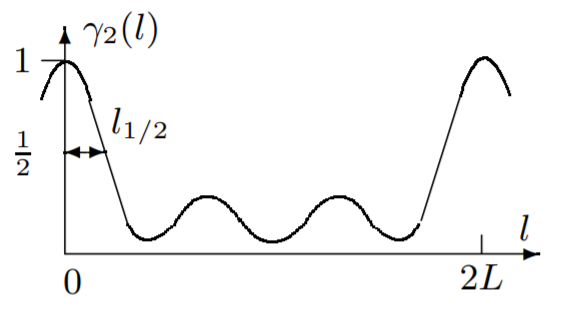
\includegraphics[scale=0.6]{1.png}
\end{center}
\caption{Зависимость $\gamma_2(l)$.}
\end{figure}
\noindent Приблизим $\gamma_2$ вблизи максимума
$$
\gamma_2 = e^{-\left(\frac{\pi \Delta F l}{c}\right)^2}
$$
Таким образом, ма имеем гауссову зависимость видности от разности хода $\gamma_2(l)$ с полушириной 
\begin{equation}
l_{1/2} = \dfrac{c}{\pi \Delta F}\sqrt{\ln 2} \approx \dfrac{0.26 c}{\Delta F}.
\end{equation}
Величина $\gamma_3$ соответсвует тому факту, что при интерференции поляризованных волн интерфирируют лишь компоненты, поляризованные одинкаово. ПУсть $\alpha$ -- угол между плоскостями поляризаций волн, тогдв
\begin{equation}
\gamma_3 = |\cos \alpha|.
\end{equation}
\section*{Установка}
\begin{figure}[H]
  \centering
  \begin{minipage}[b]{0.45\textwidth}
    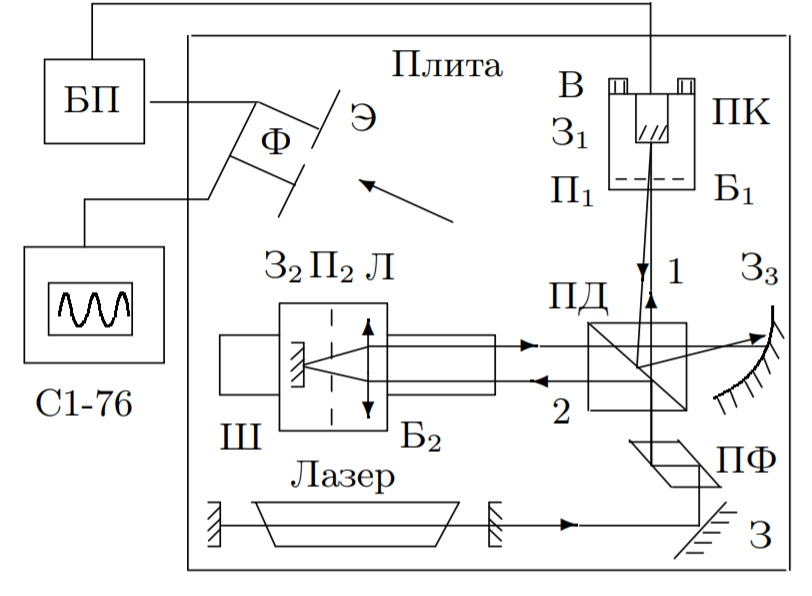
\includegraphics[width=\textwidth]{2.png}
    \caption{Схема установки}
  \end{minipage}
  \hfill
  \begin{minipage}[b]{0.45\textwidth}
    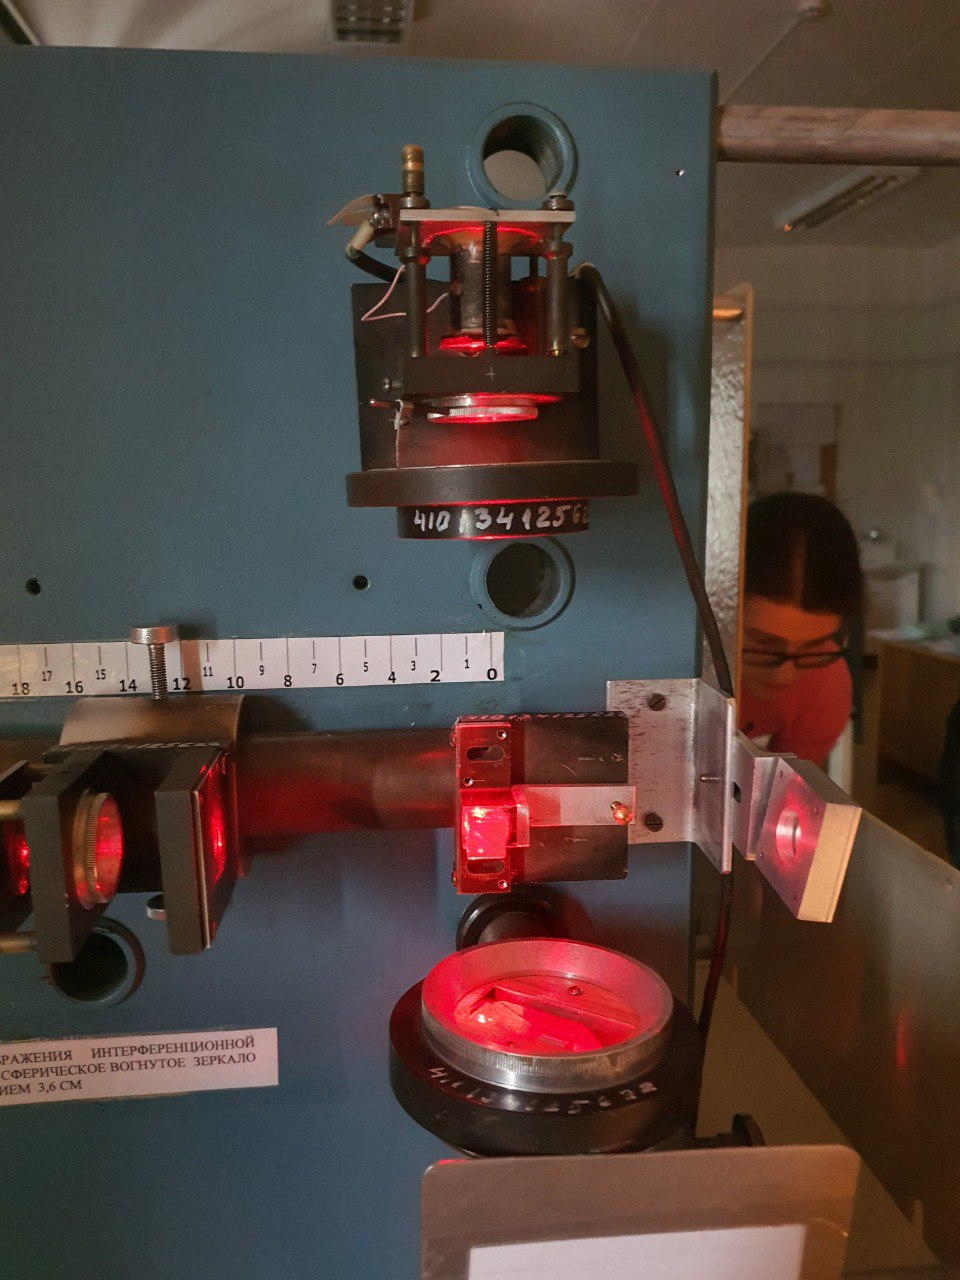
\includegraphics[width=\textwidth]{e1.jpg}
    \caption{Фотография установки}
  \end{minipage}
\end{figure}
\noindent В работе используется интерферометр Майкельсона, схема работы которого представлена на рис. 2. При этом для регистрации фоновой засветки, интенсивности света пучков, максимумов и минимумов интерференционной картины используется осциллограф, на котором наблюдается осциллограма, представленная на рис. 3.
\begin{figure}[H]
\begin{center}
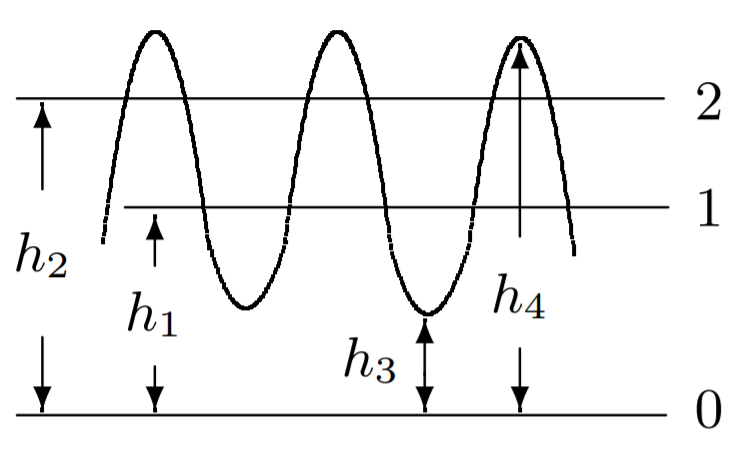
\includegraphics[scale=0.5]{3.png}
\end{center}
\caption{Осциллограмма сигналов фотодиода.}
\end{figure}
\noindent Здесь 0 -- уровень при отсутствии лучей, 1 и 2 -- при закрытии одного из них. \\
По картине на экране осциллографа можно определить параметры видимости по следующим формулам:
\begin{equation}
\delta = \dfrac{h_1}{h_2},
\end{equation}
\begin{equation}
\gamma = \dfrac{h_4 - h_3}{h_4 + h_3},
\end{equation}
При условии одинаковой поляризации лучей ($\alpha = 0$),
\begin{equation}
\gamma_2 = \dfrac{\gamma}{\gamma_1}.
\end{equation}
Если же разность хода отсутствует, то
\begin{equation}
\gamma_3 = \dfrac{\gamma}{\gamma_1}.
\end{equation}
\section*{Ход работы}
Установим дополнительный поляроид между лазером и параллелепипедом Френеля. Поворачивая его, наблюдаем, что лазер дает линейно поляризованный свет. Таким же образом пронаблюдаем за лучом, разместив поляроид между параллелепипедом Френеля и кубиком. Видим, что этот луч имеет круговую поляризацию. \\
Поворачивая $\Pi_1$, установим минимальную четкость интерференционной картины. Введем дополнительный поляроид в луч, идущий на экран. При этом на экране вновь возникает интерфереционная картина, так как после прохождения второго поляроида оба луча будут иметь одинаковую поляризацию, задаваемую поляроидом.\\
Исследуем зависимость видности интерфереционной картина от угла $\alpha$ поворота поляроида $\Pi_1$. Результаты измерений представлены в таблице 1.

\begin{table}[H]
\begin{tabular}{|c|c|c|c|c|c|c|c|} \hline
$\alpha, ^\circ$ & $h_1$, дел & $h_2$, дел & $h_3$, дел & $h_4$, дел & $\gamma_3$ & $\gamma_3 / \gamma_3(0)$ & $\sigma_{\gamma_3}$ \\ \hline
0 & 39 & 20 & 7 & 46 & 0.78 & 1.00 & 0.04 \\ \hline
10 & 42 & 19 & 8 & 44 & 0.75 & 0.96 & 0.04 \\ \hline
20 & 45 & 18 & 10 & 47 & 0.72 & 0.92 & 0.03 \\ \hline
30 & 45 & 17 & 11 & 43 & 0.66 & 0.85 & 0.04 \\ \hline
40 & 36 & 15 & 12 & 36 & 0.55 & 0.71 & 0.04 \\ \hline
50 & 30 & 15 & 12 & 31 & 0.47 & 0.60 & 0.04 \\ \hline
60 & 25 & 15 & 11 & 27 & 0.43 & 0.56 & 0.04 \\ \hline
70 & 18 & 15 & 10 & 22 & 0.38 & 0.48 & 0.05 \\ \hline
80 & 15 & 14 & 11 & 20 & 0.29 & 0.37 & 0.05 \\ \hline
90 & 9 & 13 & 10 & 16 & 0.23 & 0.30 & 0.05 \\ \hline
100 & 8 & 13 & 13 & 19 & 0.19 & 0.25 & 0.05 \\ \hline
110 & 6 & 11 & 15 & 19 & 0.12 & 0.16 & 0.05 \\ \hline
120 & 6 & 12 & 14 & 17 & 0.10 & 0.13 & 0.05 \\ \hline
130 & 5 & 11 & 15 & 17 & 0.07 & 0.09 & 0.05 \\ \hline
\end{tabular}
\centering
\caption{Результаты измерений $\gamma_3$.}
\end{table} 

\noindent Представим результаты на графике , представленном на рис. 4. Видим, что теоретическая зависимость (6) действительно выполняется. На график представлена зависимость $\gamma_3 / \gamma_3(0)$ от $\cos \alpha$, то есть значение $\gamma_3(0)$ принято за 1, чтобы исключить влияние $\gamma_2$ на результат.

\begin{figure}[H]
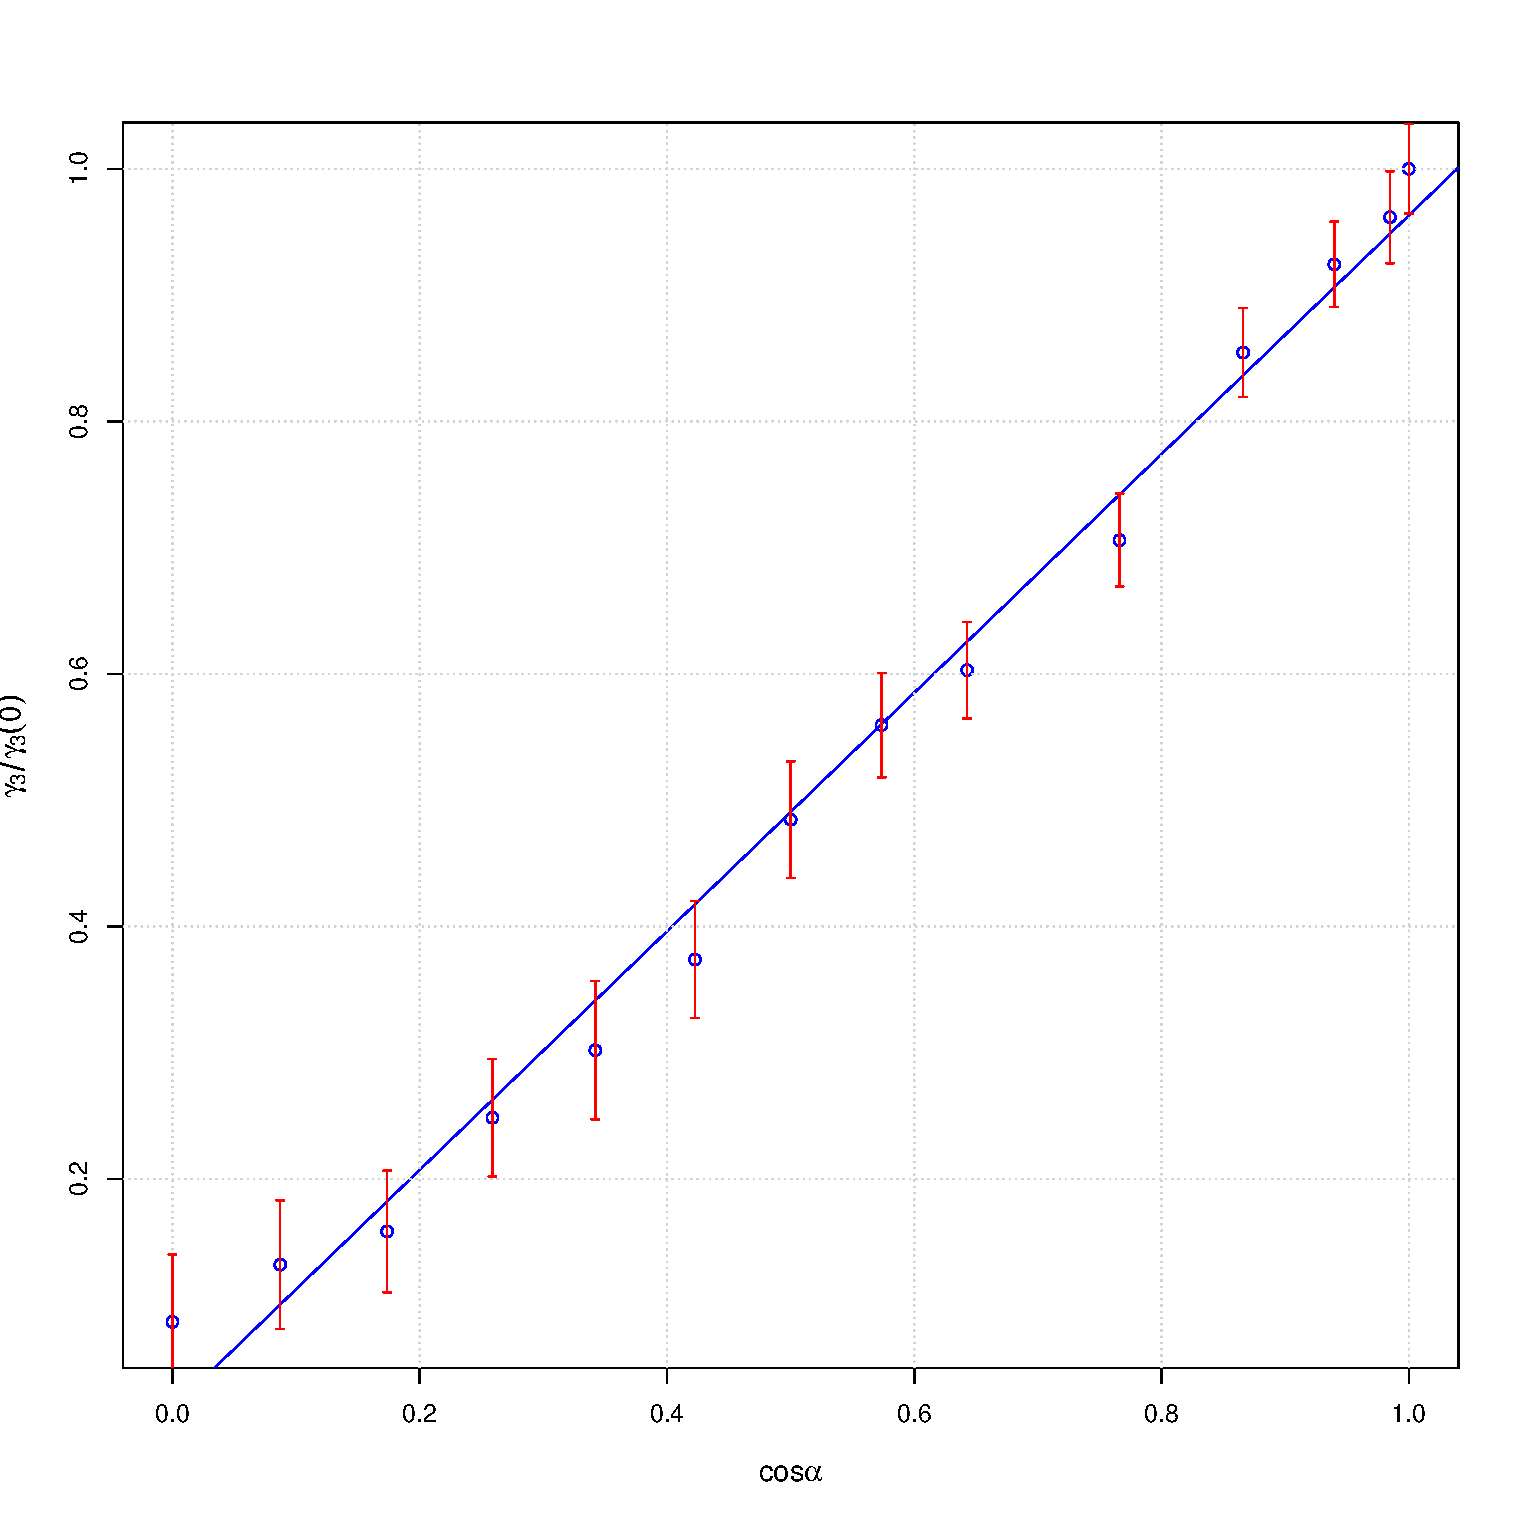
\includegraphics[scale=0.4]{g1.pdf}
\centering
\caption{Зависимость $\gamma_3(\cos \alpha)$.}
\end{figure}

\noindent Теперь исследуем зависимость видимости от разности хода между лучами. Для этого будем перемещать блок $\text{Б}_2$, координата $x$ которого и будет определять разность хода. Значения измерений представлены в таблице 2. Также по экспериментальным данным построен график, изображенный на рис. 5.\\

\begin{figure}[H]
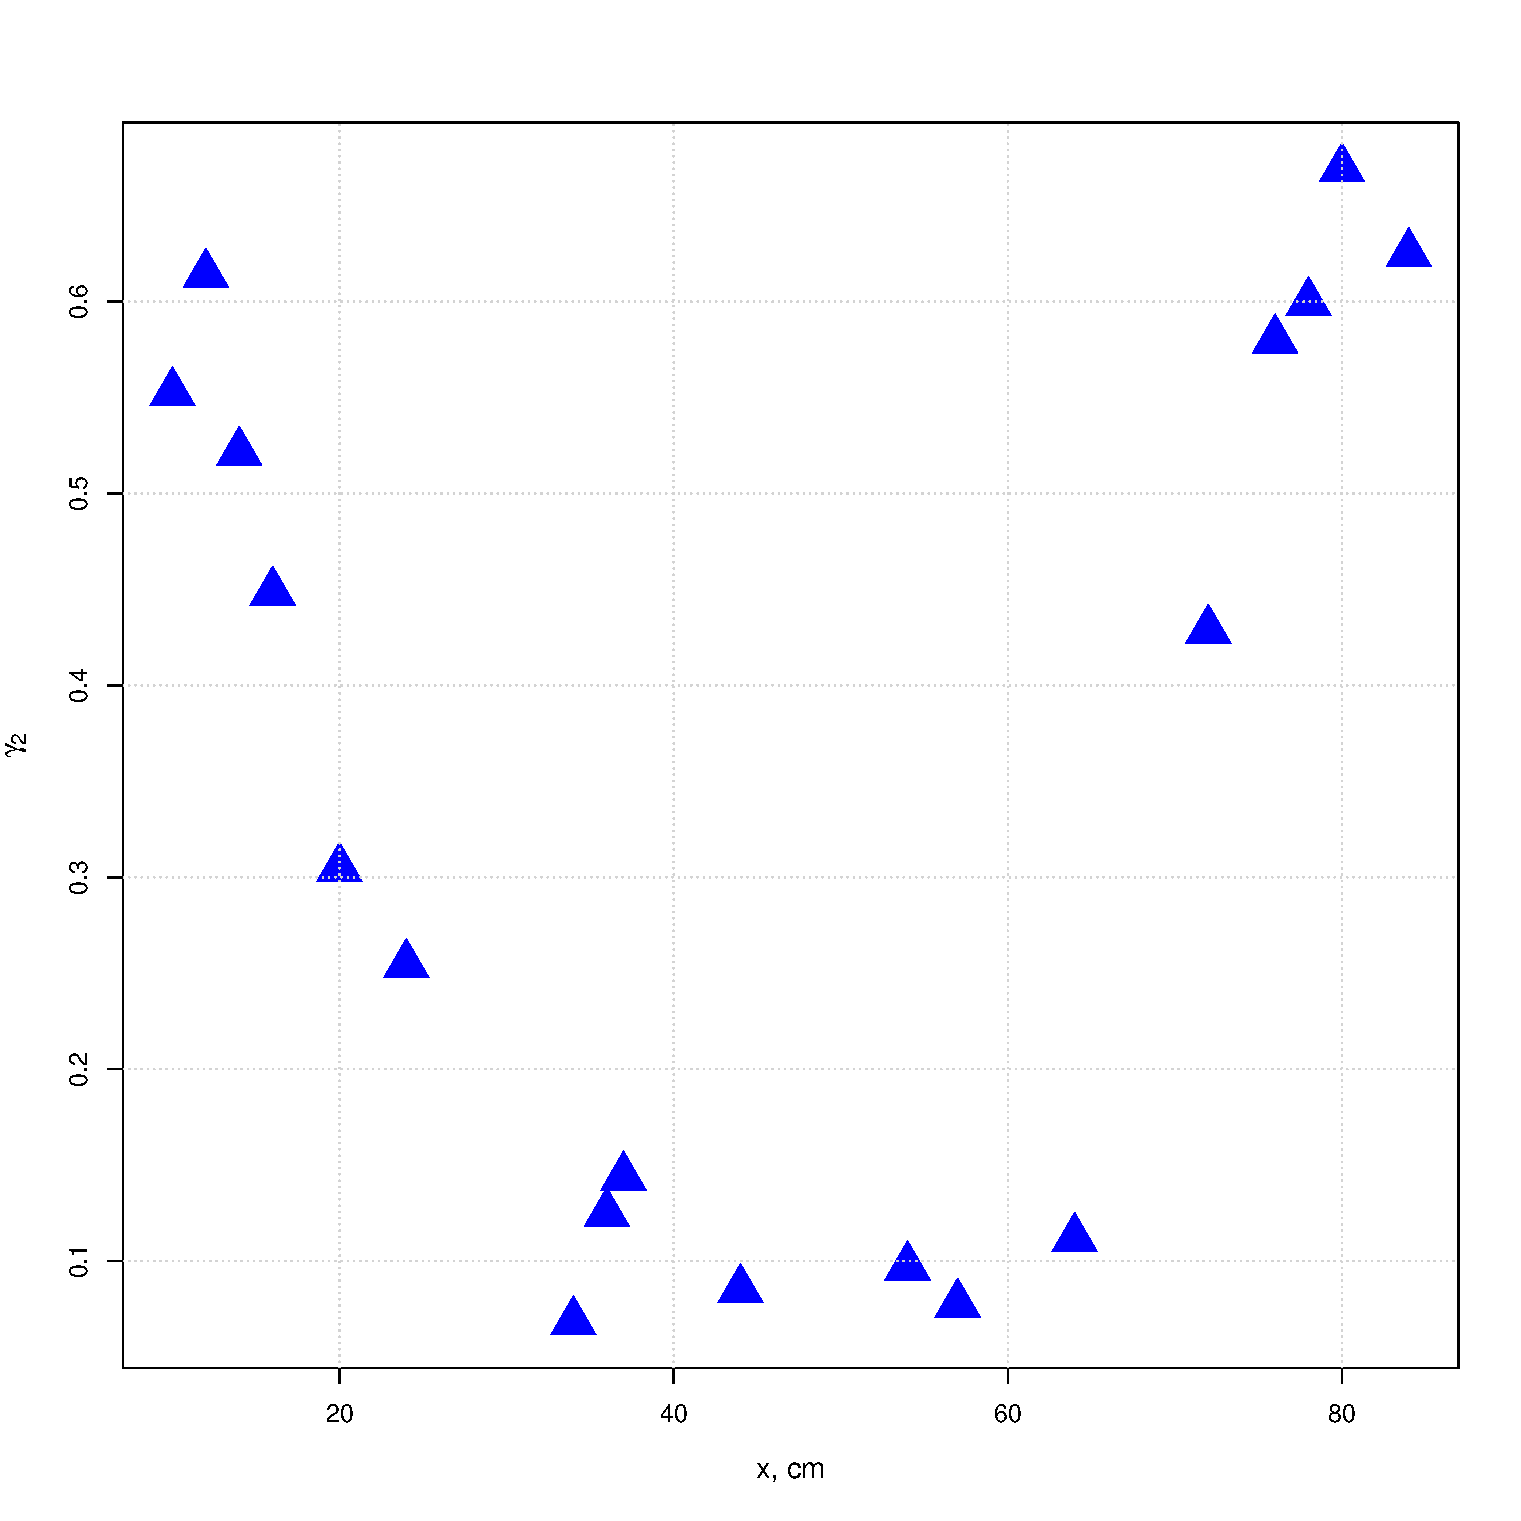
\includegraphics[scale=0.4]{g2.pdf}
\centering
\caption{Зависимость $\gamma_2(x)$.}
\end{figure}
\begin{table}[H]
\begin{tabular}{|c|c|c|c|c|c|}
\hline
$x$, см & $h_1$, дел & $h_2$, дел & $h_3$, дел & $h_4$, дел & $\gamma_2$ \\ \hline
10 & 8 & 40 & 10 & 24 & 0.55 \\ \hline
12 & 8 & 34 & 22 & 63 & 0.61 \\ \hline
14 & 4 & 38 & 34 & 64 & 0.52 \\ \hline
16 & 10 & 48 & 40 & 81 & 0.45 \\ \hline
20 & 12 & 44 & 36 & 60 & 0.30 \\ \hline
24 & 23 & 13 & 34 & 56 & 0.25 \\ \hline
34 & 46 & 15 & 32 & 36 & 0.07 \\ \hline
36 & 48 & 18 & 40 & 50 & 0.12 \\ \hline
37 & 45 & 17 & 34 & 44 & 0.14 \\ \hline
44 & 24 & 16 & 22 & 26 & 0.09 \\ \hline
54 & 9 & 37 & 24 & 28 & 0.10 \\ \hline
57 & 22 & 28 & 24 & 28 & 0.08 \\ \hline
64 & 22 & 27 & 24 & 30 & 0.11 \\ \hline
72 & 21 & 20 & 24 & 60 & 0.43 \\ \hline
76 & 22 & 29 & 20 & 74 & 0.58 \\ \hline
78 & 23 & 14 & 18 & 68 & 0.60 \\ \hline
80 & 24 & 14 & 14 & 65 & 0.67 \\ \hline
84 & 23 & 18 & 15 & 64 & 0.62 \\ \hline

\end{tabular}
\centering
\caption{Результаты измерений $\gamma_2$.}
\end{table}

\noindent На графике выделяются два максимума --- $x_1 = 12\pm2$ см и $x_2 = 80\pm2$ см. Отсюда 
$$
L = 34\pm1.4 \text{ см}
$$
$$
\Delta \nu = (4.4 \pm2 \cdot 10^8) \text{ Гц}.
$$
Также по графику определяем полуширину кривой
$$
l_{1/2} \approx 8 \text{ см},
$$
Тогда из формул (5) и (2) соответственно 
$$
\Delta F \approx 9.9 \cdot 10^8 \text{ Гц}.
$$
$$
N = 5\pm1, 
$$

\section*{Вывод}
В работе были исследованы 
\begin{enumerate}
    \item зависимость видности интерференционной картины от поляризации интерферирующих лучей. При этом была экспериментально подтверждена формула $\gamma_3 = |\cos \alpha|$ при $\alpha \in [0; \pi/2]$, где $\gamma_3$ -- видность, $\alpha$ -- угол между плоскотями поляризации.
    \item зависимость видности интерференционной картины от разности хода лучей. При этом 
\end{enumerate}

\noindent Также была экспериментально оценены такие характеристики лазера, как половина диапазона генерируемых частот и число продольно генерируемых мод соответственно
$$
\Delta F \approx 9.9 \cdot 10^8 \text{ Гц}.
$$
$$
    N = 5\pm1
$$

\end{document}


